\documentclass[11pt]{beamer}
\graphicspath{{Images/}{./}} % Specifies where to look for included images (trailing slash required)
\usepackage{booktabs}
\usetheme{Madrid}
\usefonttheme{default}
\useinnertheme{circles}

\title[GNN Interpretation]{GNN Interpretation Thesis Project} % The short title in the optional parameter appears at the bottom of every slide, the full title in the main parameter is only on the title page
\author[Shalin Patel]{Shalin Patel} % Presenter name(s), the optional parameter can contain a shortened version to appear on the bottom of every slide, while the main parameter will appear on the title slide
\date[\today]

%----------------------------------------------------------------------------------------

\begin{document}

\begin{frame}
	\titlepage
\end{frame}

\section{Introduction}

\begin{frame}
    \frametitle{GNNs and Computational Biology}

    \begin{itemize}
        \item GNNs useful for creating multi-modal models of complex biological systems (e.g. Gene Expression)
        \begin{itemize}
            \item Based off HiC contact data
            \item Based off Gene Regulatory Networks (GRNs)
        \end{itemize}
        \item These models often demonstrate state of the art performance
        \item Many biological datasets demonstrate graphical structure and are often coerced into unnatural forms
        \begin{itemize}
            \item GNNs remove a lot of these issues
        \end{itemize}
    \end{itemize}
\end{frame}

\begin{frame}
    \frametitle{Interpretation of GNNs}
   
    \begin{itemize}
        \item While GNNs give better performance than previous models, interpretating them is harder than before
        \item Many traditional models have well established interpretations
        \begin{itemize}
            \item SVMs, Random Forests, Logistic Regression all have natural interpretations
            \item CNNs also have many interpretation methods including saliency maps, LIME, SHAP, \dots
        \end{itemize} 
        \item To derive understanding, and new biological value from the improved performance, interpretations for GNNs need to be generated
        \item Specifically, we want to understand what parts of the underlying graph structure are driving newfound performance
    \end{itemize}
\end{frame}

\section{Problem Formulation and Previous Work}
\begin{frame}
    \frametitle{Problem Formulation}

    Let $\mathcal{G}$ denote a graph on edges $E$ and nodes $V$ such that each node is associated with $\mathcal{X} = \{x_1, \dots, x_n\}$.

    \bigskip

    Let $f : V \mapsto \{1, \dots, C\}$ represent a classification task on nodes in $V$. 

    \bigskip
    
    Specifically, for a node $v$, a GNN $\phi$ that approximates $f$ learns the conditional distribution $P_{\phi}(Y \mid G_c(v), X_c(v))$ where $G_c$ and $X_c$ represent the computaitonal graph of $v$ (typical the $n$-hop neighborhood). Predictions are given as $\hat{y} = \phi(G_c(v), X_c(v))$.

    \bigskip

    The goal of GNN interpretation is to find $\psi : V \mapsto \mathcal{G}$ where $\psi(v) = G_s(v)$ such that $G_s(v) \subseteq G_c(v)$ and
    \[
        MI(\hat{y}, \phi(G_s(v), X_c(v))) 
    \]
    is maximized.
\end{frame}

\begin{frame}
    \frametitle{GNNExplainer}

    \begin{itemize}
        \item GNNExplainer works by learning a continuous mask $\sigma(M)$ such that $A_c \odot \sigma(M)$ represents the interpretation
        \item GNNExplainer assumes $P_{\mathcal{G}}(G_S) = \prod_{(j,k) \in G_c} A_s[j, k]$ meaning that each edge is treated as an independent Bernoulli RV
        \item This mask is learnt via backpropogation on the mutual information with respect ot these $A_s[j, k]$. 
        \item In practice, this ignores all sorts of conditionality between the edges and is not rich enough to capture complex interactions between edges
        \begin{itemize}
            \item Does not perform well in replicaiton studies
            \item Has extremely high variance and does not converge consistently
        \end{itemize}
    \end{itemize}
\end{frame}

\begin{frame}
    \frametitle{PGExplainer}

    \begin{itemize}
        \item The current SOTA (based on some flawed benchmarks)
        \item Has about 0.78 AUC in replication studies
        \item Requires a split between graph embedding and inference model to work
    \end{itemize}
\end{frame}

\begin{frame}
    \frametitle{Benchmark Dataset}
    
    \begin{center}
        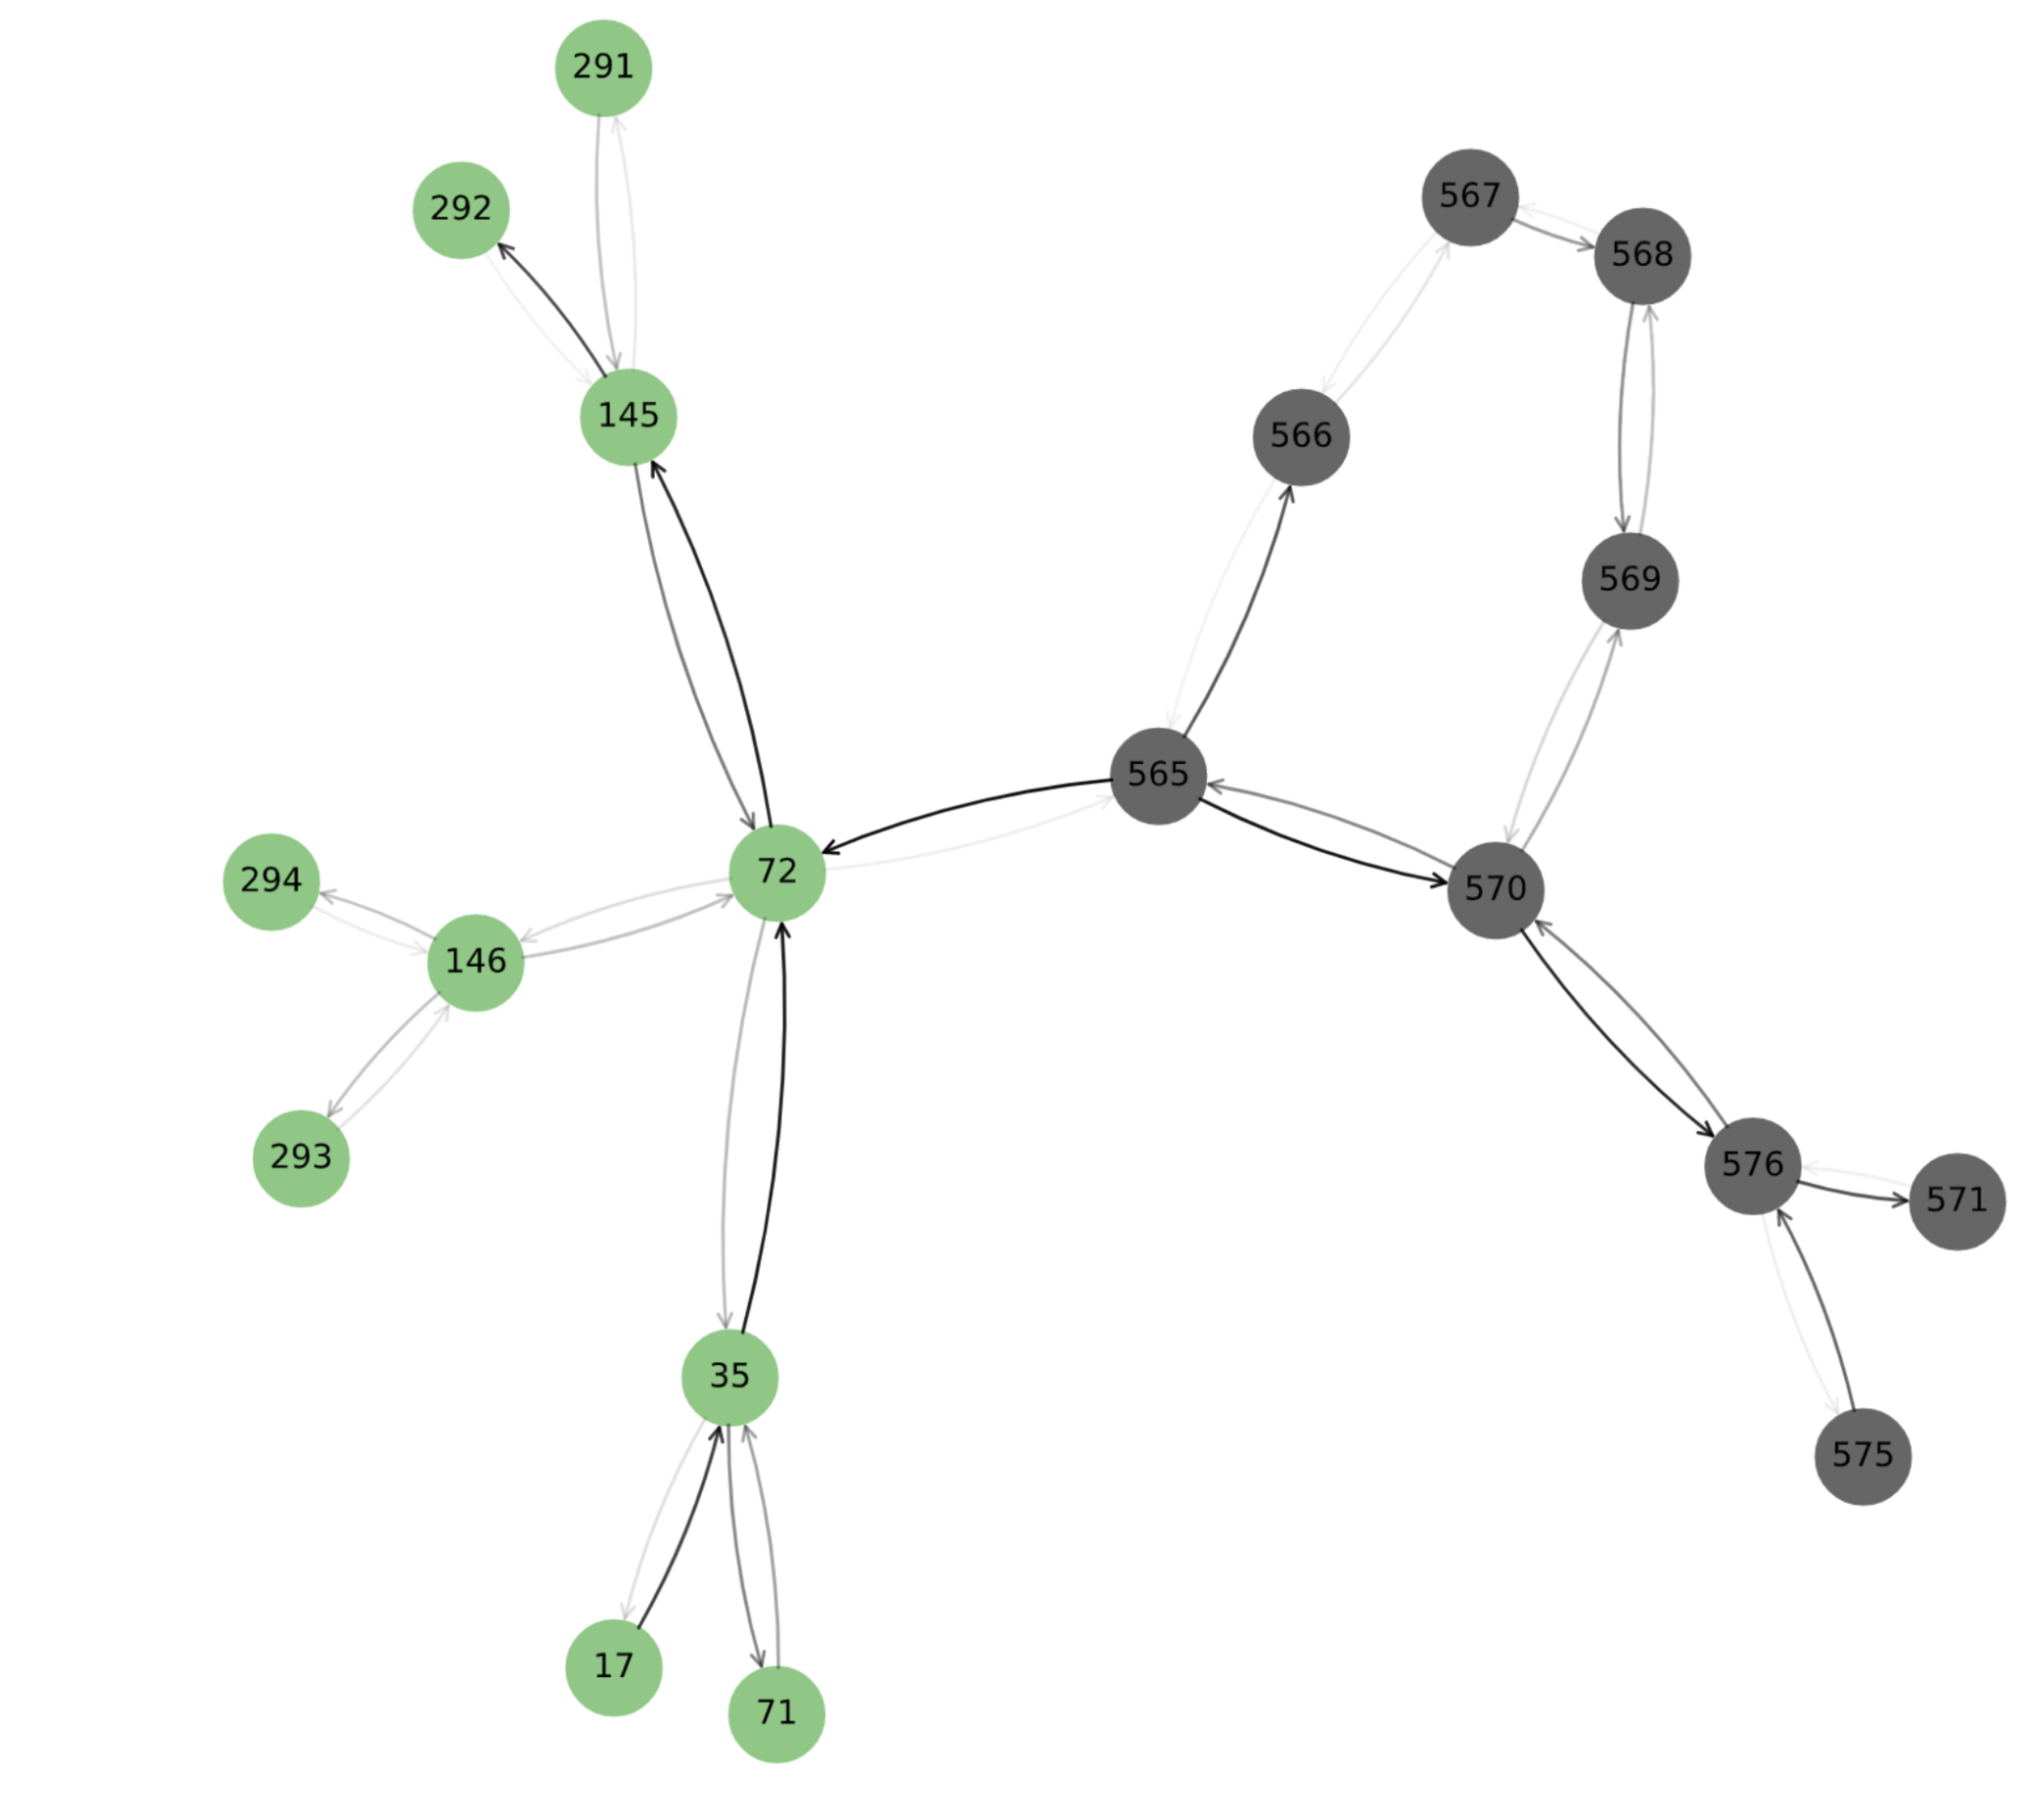
\includegraphics[width=0.75\textwidth]{tree_cycles.png}
    \end{center}
\end{frame}

\section{Bayesian Approach}
\begin{frame}
    \frametitle{Bayesian Formulation}

    \begin{itemize}
        \item Specify a model $\bar{\psi}$ for sampling $G_s(v)$
        \item Given a mask $M$ sampled from this distribution, condition $\phi(M, X_c(v))$ on $\phi(G_c(v), X_c(v))$ and update the parameters of $\bar{\psi}$ using SVI
        \item There are many different models we can try
        \item We want a good tradeoff between structure and flexibility to capture the complex conditional interactions that are happening in the underlying dataset
    \end{itemize}
\end{frame}

\section{Current Attempts}
\begin{frame}
    \frametitle{Beta-Bernoulli Model}
    \begin{itemize}
        \item Sampled each edge from a Beta-Bernoulli variable with the following prior on a given edge \\
        \begin{center}
            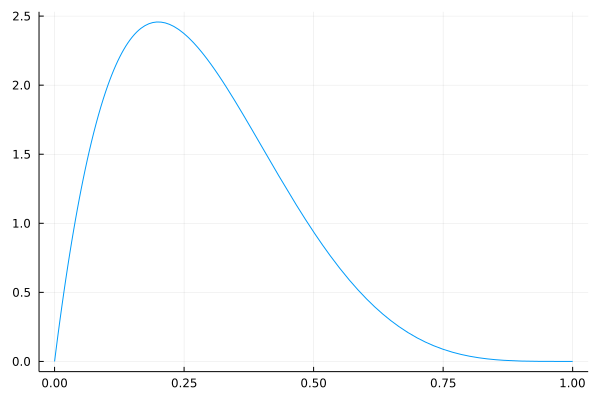
\includegraphics[width = 0.5\textwidth]{beta_bernoulli.png}
        \end{center}
        \item Does not perform super well $\sim$ on par with GNNExplainer (makes sense these are essentially the same model)
    \end{itemize}
\end{frame}

\begin{frame}
    \frametitle{Random Walk Model}

    \begin{itemize}
        \item Worked by randomly choosing an node adjacent to $v$
        \item Sampled edges in the set adjacent to all added nodes and continued until no more nodes to add with each edge being drawn from an independent Bernoulli distribution
        \item Performed a bit better reaching $\sim$ 0.55 AUC
    \end{itemize}
\end{frame}

\begin{frame}
    \frametitle{Normalizing Flow Model}

    \begin{itemize}
        \item If there are $e$ edges in $G_c(v)$, we have an $e$-dimensional base mv-normal distribution
        \item Uses and invertible spline transform-based normalizing flows to transform base distribution to a target distribution over all edges
        \item Sampled from this target distribution to build an edge mask
        \item Gives the most flexibility
        \item Performs around $\sim$ 0.60 AUC
    \end{itemize}
\end{frame}

\section{Conclusion}
\begin{frame}
    \frametitle{Next Steps}

    \begin{itemize}
        \item Defintely have some bugs that are leading to suboptimal training
        \item Reevaluate how to evaluate these models
        \item Evaluate PGExplainer against actual ground truth examples
        \item Explore different transforms in the normalizing flow model
        \item Combine random walk with normalizing flow
    \end{itemize}
\end{frame}

\end{document}